\section{Hauptteil}
\subsection{Resultat}

Resultat ist eine Webapp, welche in allen modernen Webbrowsern funktioniert. Mittels Klicken können Start- \& Zielpunkt ausgewählt werden. Mit einem bestätigenden Klick auf <<Ausführen>> wird im Hintergrund ein GIS-Modell gestartet, welches entweder eine <<rohe>> Gefahrenkarte oder eine mit eingebrannten Gewässern verwendet.

\subsubsection{Modellevaluation}

Es wurden 14 typische Frühlings-Skitouren \& -Skihochtouren aus dem SAC Tourenportal ausgewählt und mittels einem kurzen Python-Skript heruntergeladen. Anschliessend wurden die Modellversionen mit und ohne eingebrannten Gewässern für die Start und Zielpunkte der einzelnen Routensegmente ausgeführt. Star und Zielpunkte wurden dabei von Hand plaziert. Für alle 28 Tests wurden die Gleichen Hyperparameter verwendet: $k_{risk}={50.0};\ c_{steepascend}={5.0};\ c_{steepdescend}={5.0};\ c_{flat}={0.25};\ c_{ascend}={2.5};\ c_{descend}={2.5}$

Für einige Regionen bzw. Gipfel (Länta, Steingletscher) war nur eine von beiden Gefahrenkarten brauchbar --- so macht es wenig Sinn, Quer über den Steinsee zu laufen, da dieser nur selten zugefroren ist. Erfahrungswerte mit beiden Modellversionen zeigen, dass in den meisten Fällen beide Versionen vom Benutzer begutachtet werden müssen.

%TOUREN
%// Clariden
% //Galenstock
% //Dammastock
% //Rheinwaldhorn
%// Dufourspitze
% // Signalkuppe
% // Piz Palü
%// Tierbergli
%// Sustenhorn

Nachfolgend wird eine Auswahl der Touren kurz diskutiert. Mit eigenen Touren kann auf \url{https://algotour.app} experimentiert werden.

Die besten Routen waren jene vom Steingletscher aus auf die Tierberglihütte SAC, sowie auf das Sustenhorn. (Wenn die korrekte Gefahrenkarte verwendet wird --- Die andere produziert unbrauchbare Resultate) Es kann eine hohe Korrelation mit den Literaturrouten die der SAC im Tourenportal auflistet festgestellt werden~\cite{mmzentralch}. (Siehe Abb.\ \ref{fig:tierbergli})

Ebenso erreicht die Tour auf den Clariden in der Eigenevaluation eine Bestnote --- Hier trumpft jedoch die nicht mit Gewässern ergänzte Karte (Siehe Abb.\ \ref{fig:clariden}). Die nicht ganz offensichtliche Gratpassagen werden vom Modell sehr gut abgebildet, der Bach an einem sinnvollen Ort überquert. Die Übereinstimmung mit der SAC-legitimierten Route ist ebenfalls hervorragend~\cite{twslstgallappzll}.

Weniger erfreulich sieht das Resultat bei den Touren im Monte Rosa Massiv aus. Bei der Route auf die Dufourspitze findet der Algorithmus ohne weitere Hilfe zwar eine Spuranlage, welche als Hochtour so existiert, im Winter jedoch --- dank einer Kletterstelle im~\rom{3}. Grad --- kaum oder nur unter extremer Schwierigkeit und nur ohne Skis begangen werden kann. 
Die Tour welche nicht direkt zum Gipfel, sondern nur bis zum Skidepot der Literaturtour führt, funktioniert und kann so begangen werden. Die Routenwahl ist jedoch um einiges defensiver als jene aus dem Tourenführer (siehe Abb.\ \ref{fig:monterosa} <<Manuelles Skidepot>>). Ein umweg von ca.\ \qty{1}{h} wird gegenüber eines \qty{32}{°} steilen Hanges in Kauf genommen.

Die Route auf den Piz Palü ist aufgrund der Nähe zu einer Spaltenzone (siehe Abb.\ \ref{fig:pizpalu}) nur bei günstigen Wetterverhältnissen zu empfehlen --- in einem schneearmer Winter sind Schneebrücken über Spalten beispielsweise grundsätzlich schwächer~\cite{bergsteigenErhhtesRisiko}. Sie kann jedoch ansonsten ohne grössere alpintechnische Probleme begangen werden.

Auch bei den Touren auf den Galenstock sowie den Dammastock werden eher einer Hochtour entsprechende Spurwahlen getroffen. In der Praxis sind diese mit Skiern mangels einer attraktiven Abfahrt vom Skidepot aus keine Trendtouren-Kandidaten. (Für diese Routen siehe Anhang..........)
%TODO: Insert correct ref

\begin{Mappage}
{
  \begin{figure}[H]
    \centering
    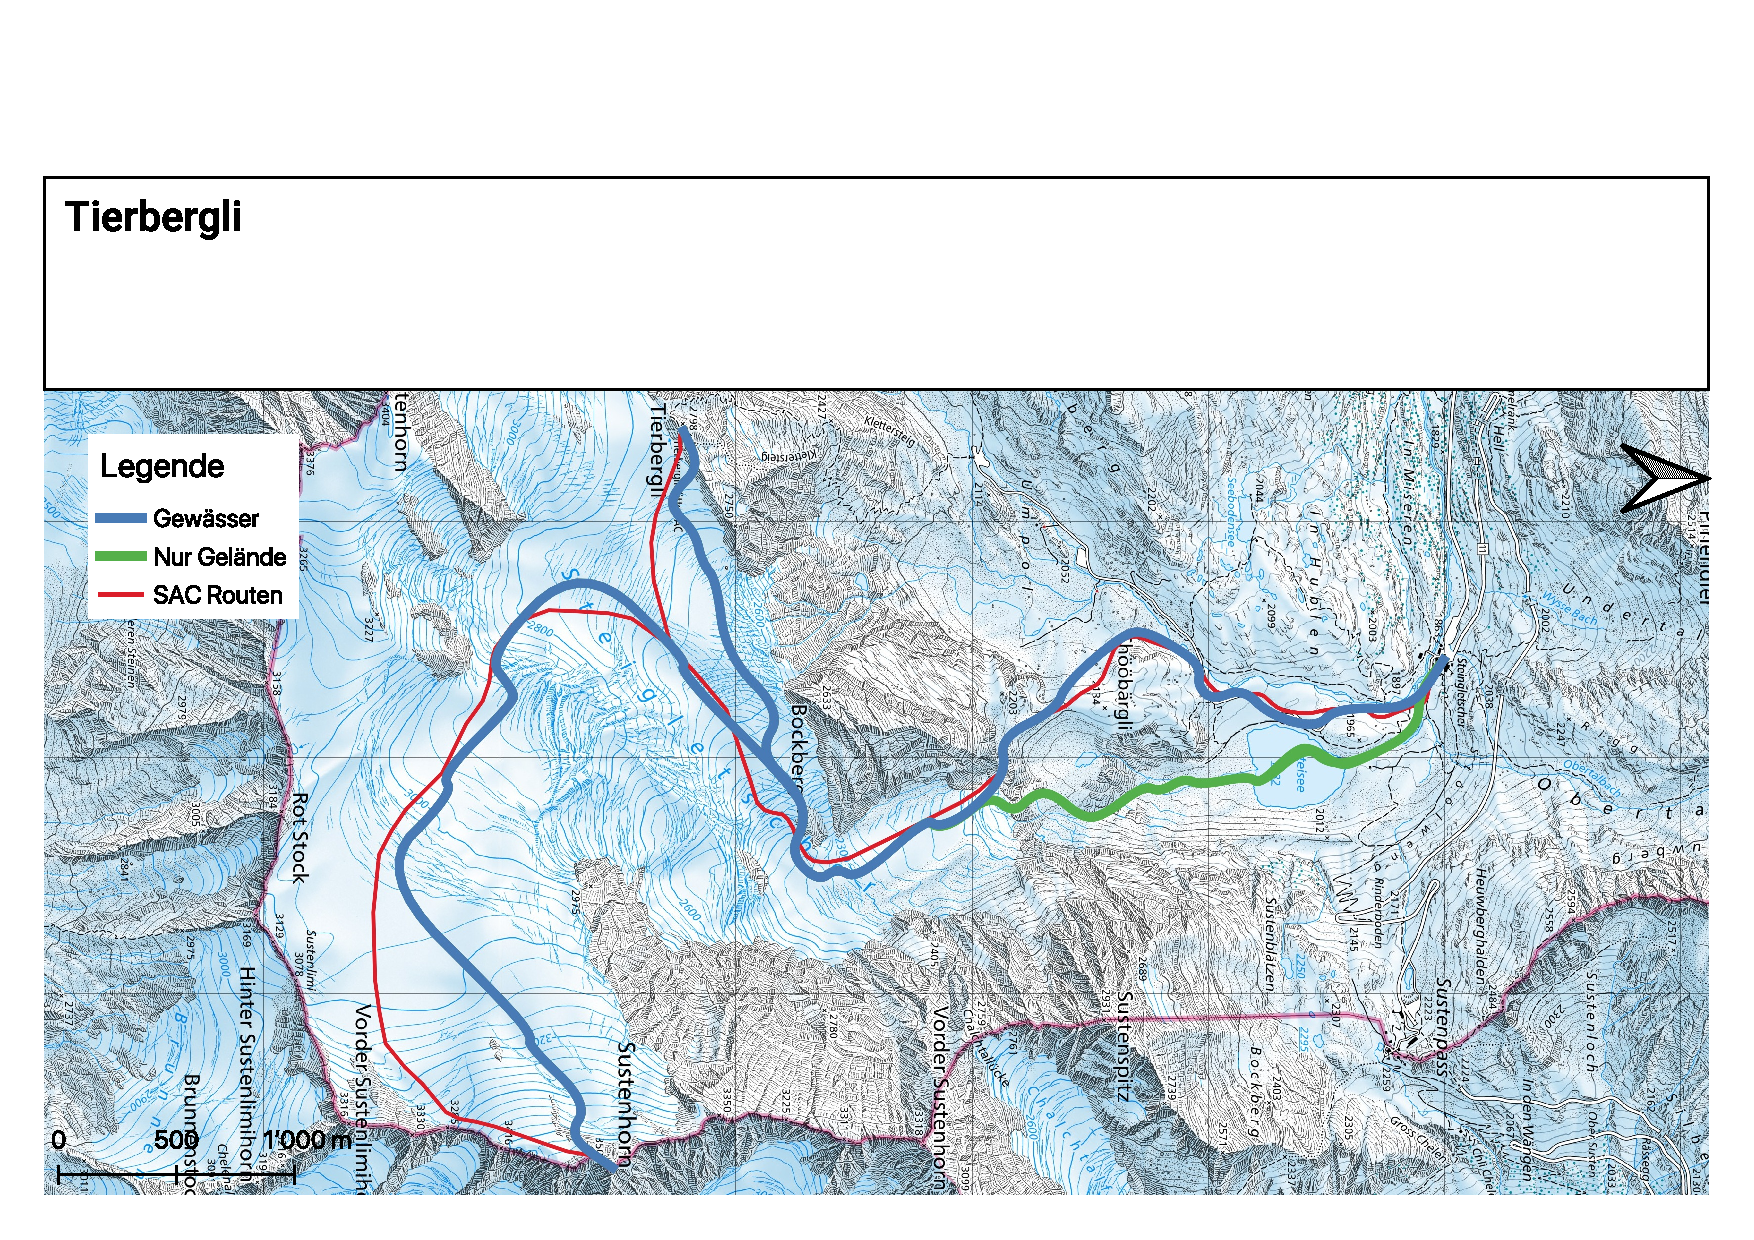
\includegraphics[page=1,width=.9\linewidth]{./../evaluation/PDFs/Tierbergli.pdf}
    \caption{Tour vom Steingletscher zu der Tierberglihütte SAC und dem Sustenhorn, \\Basislayer: swisstopo}\label{fig:tierbergli}
    \end{figure}

  \begin{figure}[H]
    \centering
    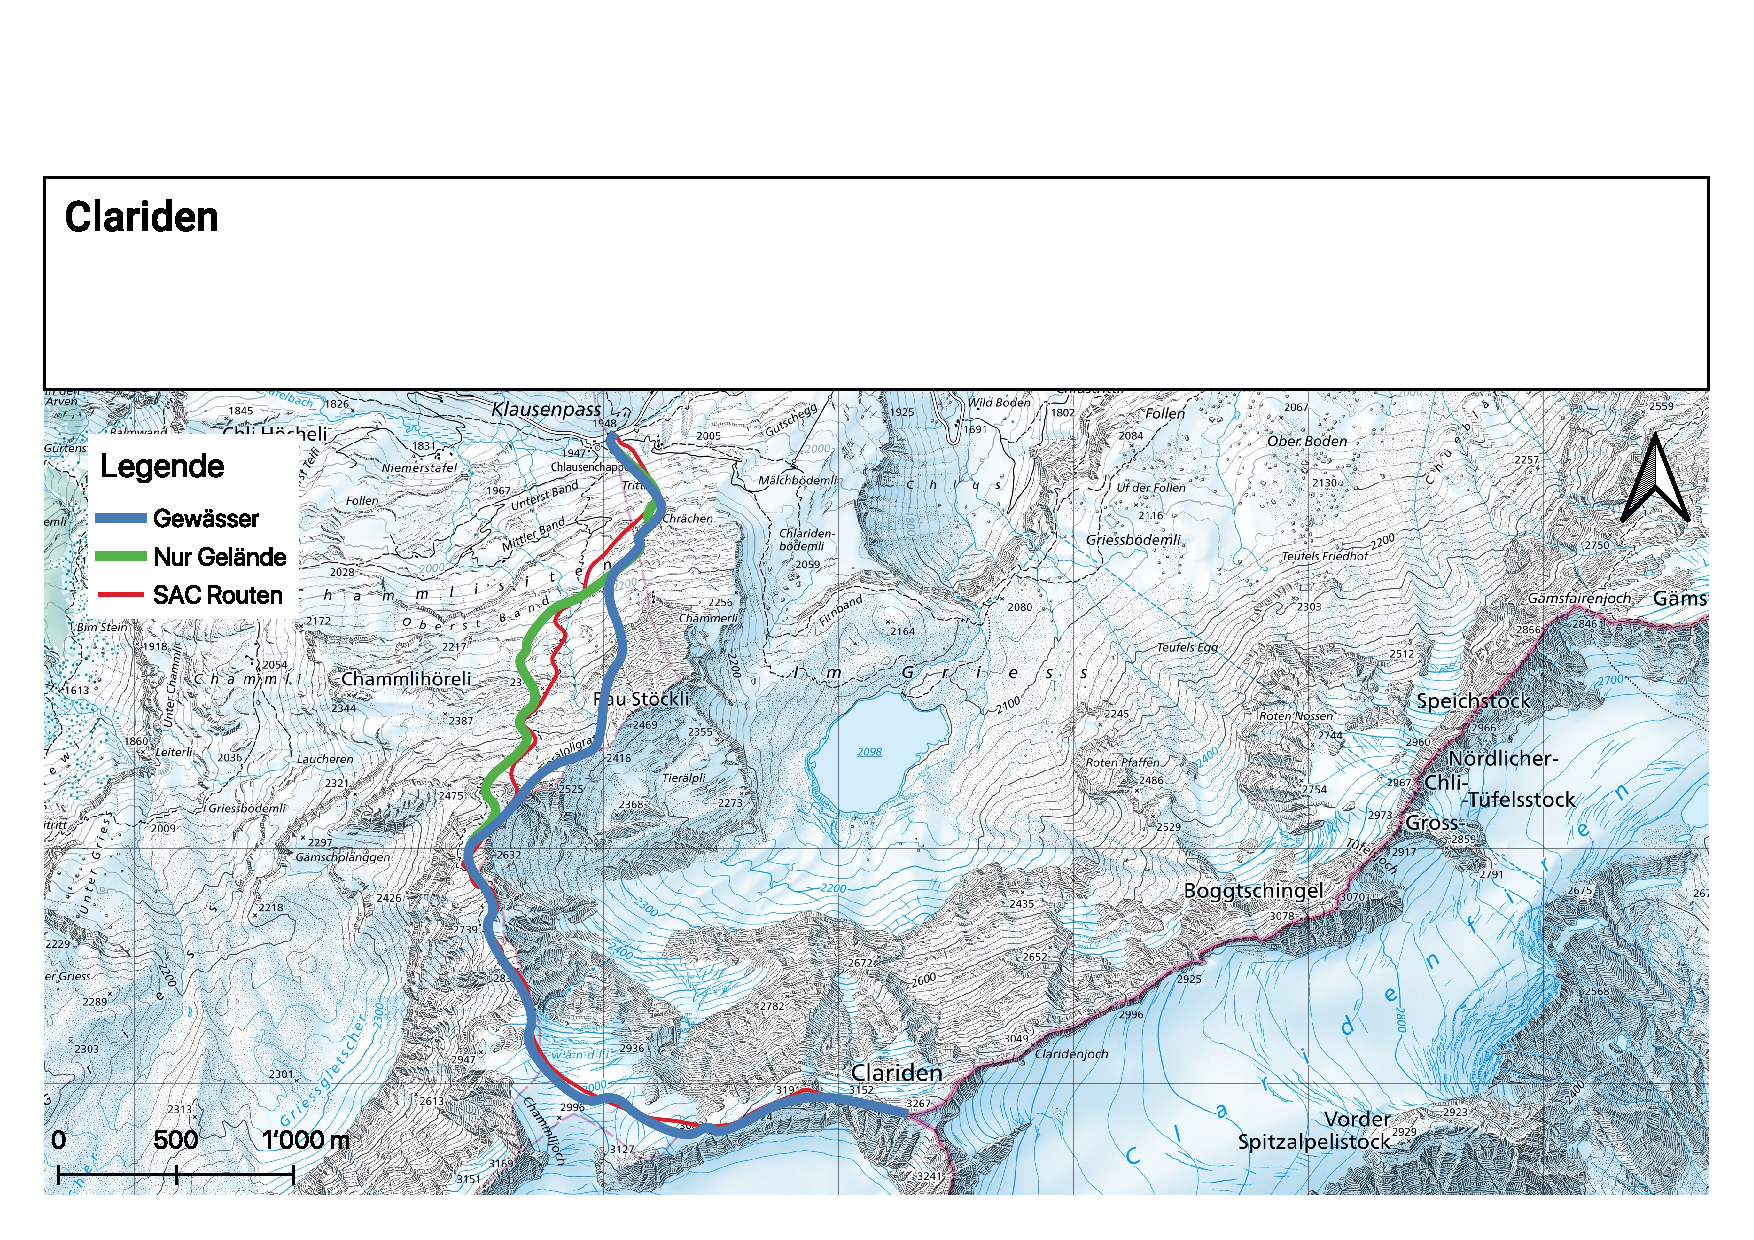
\includegraphics[page=1,width=.9\linewidth]{./../evaluation/PDFs/Clariden.pdf}
    \caption{Geplante Tour von der Klausenpass-Passhöhe auf den Clariden, \\Basislayer: swisstopo}\label{fig:clariden}
  \end{figure}
}
% \end{Mappage}

% \begin{Mappage}
{%
    \begin{figure}[H]
      \centering
      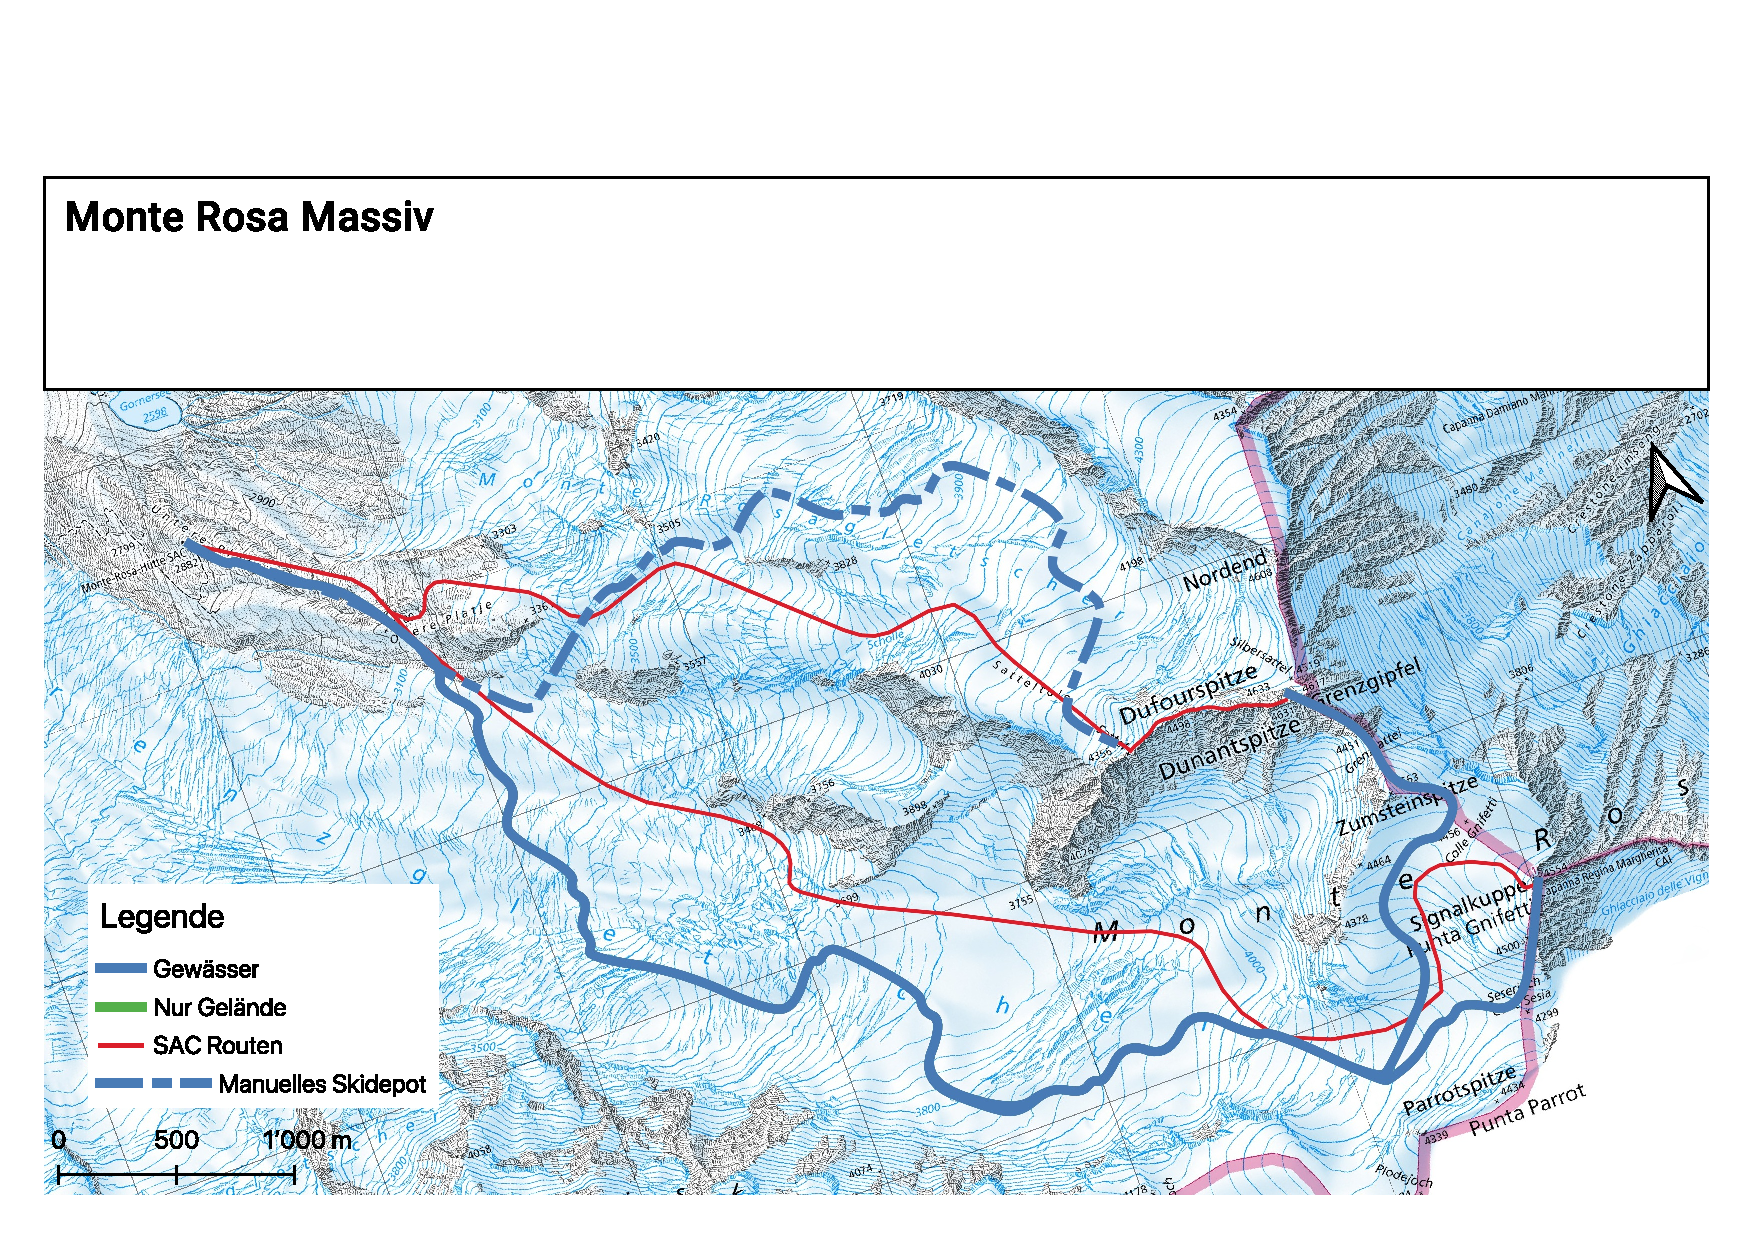
\includegraphics[page=1,width=.9\linewidth]{./../evaluation/PDFs/Monte Rosa Massiv.pdf}
      \caption{Geplante Tour von der Monte-Rosa-Hütte SAC auf Dufourspitze und Signalkuppe,\\Basislayer: swisstopo}\label{fig:monterosa}
    \end{figure}
    \begin{figure}[H]
      \centering
      \includegraphics[page=1,width=.9\linewidth]{./../evaluation/PDFs/Piz Palü.pdf}
      \caption{Geplante Tour von der Diavolezza auf den Piz Palü\\Basislayer: swisstopo}\label{fig:pizpalu}
    \end{figure}
}
\end{Mappage}

\subsection{Methodische Reflexion}
\subsubsection{Versionierung, Backup und Archiv mit Git}
\subsubsection{Verworfene Variante}
\subsubsection{GIS}
\subsubsection{Verfassen mit \LaTeX}
\subsubsection{Evaluation}

